\section{Experiment}
The here experiment mainly being investigated in the framework of this thesis was performed in $2020$ in the FAIR Phase-0 campaign at GSI (Gesellschaft f\"ur Schwerionenforschung) in Darmstadt (Germany). The GSI operates a unique accelerator facility for heavy ions and focuses on several cutting-edge research fields. These include:\newline
\begin{enumerate}
\item \textbf{Nuclear Physics}: Studying the properties of atomic nuclei, exploring the forces that bind protons and neutrons, and investigating exotic nuclei far from stability. This effort involves major international collaborations, including HISPEC/DESPEC, which investigates the structure of atomic nuclei through high-resolution spectroscopy~\cite{gerl2009nuclear},and the R$^3$B Collaboration, which focuses on kinematically complete measurements of nuclear reactions. An important aspect of this field also includes the discovery of new elements. Notably, experiments at the GSI accelerator facility have led to the identification of superheavy elements with atomic numbers 107 to 112~\cite{ackermann2007superheavy}.
\item \textbf{Hadron and Quark Matter}: Investigating the behavior of hadrons (particles made of quarks) and the state of matter under extreme conditions, such as those found in neutron stars or during the early universe, see e.g. HADES experiment \cite{galatyuk2014hades}.
\item \textbf{Atomic Physics}: Examining the structure and dynamics of atoms, including highly charged ions, to understand fundamental atomic interactions and refine quantum electrodynamics, see e.g. \cite{kluge2008hitrap}. This includes also the field of superheavy element chemistry which make nuclear studies of the heaviest man-made elements. 
\item \textbf{Plasma Physics}: Creating and analyzing high-energy-density plasmas to simulate conditions found in stellar interiors and other astrophysical phenomena, see e.g. PHELIX laser facility \cite{major2024high}.
\item \textbf{Biophysics and Medical Research}: Exploring the effects of ion beams on biological systems for applications in cancer therapy, particularly using heavy ion therapy, and studying radiation protection for space missions.
\item \textbf{Materials Research}: Investigating the response of materials to high radiation doses to develop more resilient materials for use in various technologies, including nuclear reactors and space exploration.
\end{enumerate}
\subsection{GSI facility}
The GSI Helmholtzzenrum f\"ur Schwerionenforschung GmbH was founded in 1969 (as "Gesellschaft f\"ur Schwerionenforschung mbH) looks back on a successful research history. In the time between 1981 and 2010 six new  superheavy elements were discovered\footnote{A comprehensive overview work of five decades of GSI superheavy element discoveries can be found here \cite{dullmann2022five}} \newline
In the medical research field GSI has developed advanced cancer therapy techniques using heavy ion beams which target tumors with high precision, minimizing damage to surrounding healthy tissues.\newline
Along with those groundbreaking discoveries in research the facility at GSI has always been an inspiring source of drive for new technologies.\newline
The key devices and apparatus enabling heavy-ion experiments at GSI makes it to  one of the most advanced accelerator facilities in the world.\newline
The starting point for the production of relativistic heavy ions at GSI is a set of different ion sources where ions are generated by stripping electrons off the shell of the atoms. Depending on the experimental needs the ion sources at GSI are able to produce ions of all different stable elements (up to Uranium)\cite{ion_sources_web}. The only limitations arise from safety regulations, which currently prohibit the use of toxic primary beams, such as thallium (Tl).\newline
%cite here: https://www.gsi.de/en/researchaccelerators/accelerator_facility/ion_sources
On the first acceleration stage the stable primary ions are injected from the ion source into the UNIversal Linear Accelerator (UNILAC). On a length of 120 meters ions are accelerated up to maximum energy of 11.4 AMeV. The low energy beam can be either directly used or being injected into the ring accelerator SIS18 (Schwerionensynchotron 18). Here the ion beam is further accelerated up to 4.7 GeV/u (for protons) / 1 GeV/u (for Uranium). The magnets and  the ultra-high vacuum ($\sim$ $10^{-9}$ Pa) keep the ions well on their circular path (SIS18 has a circumference of 216 meters)\cite{sis18_web}. For the production of rare heavy isotopes the primary ion beam from SIS18 can be impinged on a light nuclear target, e.g beryllium, the so called production target. The secondary beams of radioactive isotopes are typically purified in the FRagment Separator (FRS). The FRS as a high-resolution magnetic spectrometer is capable to precisely select specific isotopes and to forward the desired beam of exotic relativistic nuclei to the various experiments or direct it to the ESR for later use.\newline
%cite here: https://www.gsi.de/en/researchaccelerators/accelerator_facility/ring_accelerator
\subsubsection{FAIR Project}
The Facility for Antiproton and Ion Research (FAIR) will extend these capabilities significantly and will be one of the most advanced and extensive accelerator complexes in the world. The construction of the superconducting ring accelerator SIS100, with a circumference of 1.1 km, along with associated storage rings and experimental sites, began in the summer of 2017. The commissioning of parts of the facility is planned for 2027, followed immediately by the Early Science Program.\newline  
The so-called First Science Phase, which will mark the full operation of SIS100 and the complete commissioning of FAIR equipment, will be the next step. Prior to the commissioning of SIS100, several high-priority experiments with significant scientific impact will take place as part of the Early Science Program in the newly established experimental halls. These include experiments utilizing the R$^3$B setup in the High-Energy Cave (HEC), focusing on key aspects of nuclear structure and reactions under extreme conditions.

\subsection{R$^3$B Setup}
The R$^3$B (Reactions with Relativistic Radioactive Beams) experiment currently still operated  in Cave C at the GSI is a cutting-edge research experiment focused on the study of nuclear reactions and structure using high-energy radioactive ion beams. The experiment aims to investigate exotic nuclei far from stability, offering insights into the fundamental properties of nuclear matter, nucleosynthesis processes, and the forces governing nuclear interactions. A schematic overview of the R$^3$B setup can be seen in Figure \ref{fig:r3b_setup_intro}.\newline
\begin{figure}[htpb]
    \centering
    \includegraphics[width=\textwidth,height=6cm,keepaspectratio=true]{Figures/r3b_setup_intro.png}
    \caption{
    Overview of the R$^3$B setup in Cave C with detectors for the specific fragment branch identification.
    } 
    \label{fig:r3b_setup_intro}
\end{figure}
Short living isotopes are injected to the Cave C from the FRS, which preselects the isotopes of interest, and impinge on a fixed target. The R$^3$B setup is designed for kinematically complete reaction studies. To fulfill this requirement the incoming ions are tracked and identified on an event-by-event basis by dedicated detectors in the FRS via time-of-flight and $\Delta$E measurement techniques \cite{nociforo2014time}. Depending on the settings and composition of the incoming ion beam different type of reactions take place in the target area with a large variety of reaction products: heavy ions (as producs from fission/spallation reactions), neutrons, light charged particles and gamma rays. For the detection of gammas and light charged ions from reactions with the target the dedicated CALIFA calorimeter (see more in section \ref{sec:califa}) and various tracking detectors are installed in the target region. The GLAD (GSI Large Acceptance Dipole) magnet, located at the center of the Cave C, allows fragment identification for the forward boosted charged reaction residues. The magnetic rigidity of the charged reaction residues is measured by a combination tracking detectors and a time of flight wall after the GLAD magnet. This allows to identify the charged reaction residues and their momenta. For the detection of the neutrons, not deflected by the magnetic field of GLAD, the new Large-Area Neutron Detector (NeuLAND) is positioned after GLAD on the zero degree line with the incoming ion beam.\newline
The R$^3$B setup offers high flexibility, allowing operation both in vacuum and in atmospheric conditions. Over the past few years, during the so-called \textit{Phase-0}, numerous experiments have been conducted, each utilizing different configurations and newly developed or upgraded detector systems.\newline  
The combination of a broad spectrum of incoming ion beams across a wide energy range, provided by the FRS facility, and the versatility of the R$^3$B setup -- equipped with state-of-the-art detectors tailored for specific physics studies -- makes it an exceptional platform for experimental nuclear and astrophysics.

\subsection{Detector Setup in S444 Commmissioning Experiment 2020}
The S444 Experiment (successor experiment of the FAIR Phase-0 program in 2019, see ref. \cite{ponnath2024measurement}) for the commissioning of the CALIFA Calorimeter in its final mechanical design took place in February 2020. The choice to operate with stable $^{12}$C primary beam with four beam energy settings - 400/550/650/800 AMeV  gave the opportunity to use it as preparation for the following up S467 experimental run with neutron-rich \textit{Ca} isotopes as medium-heavy incoming beam. The detectors for ion tracking, charge identification and time of flight measurement were provided by the SOFIA(Study on Fission with ALADiN\footnote{ALADiN magnet was the precessor of GLAD.}) collaboration. These detectors are optimized for fission experiments with medium to heavy reaction fragments. As for the S444 experiment with primary $^{12}$C incoming beam no fission reaction with multiple heavy charged fragments is expected the Sofia detectors were adapted accordingly (e.g. only one of the four sections of the Twin-Music Ionisation chamber was operated, see more in section \ref{sec:ionisation_chambers}).\newline
For this experiment, most detectors and components of the setup were operated in air. The target chamber, as well as the GLAD magnet, was filled with gaseous helium at room temperature to reduce scattering of the ions.\newline 
However, the presence of gas, detectors and window material in the setup leads to ion interactions, causing angular straggling in the flight path reconstruction. This effect can limit the resolution of the reconstructed momenta from reactions occurring at the target.\newline
In the following sections the different detector components and their properties are discussed.\newline

\subsubsection{Multi Wire Proportional Chambers (MWPC)}\label{sec_mwpcs}
The positional tracking of the incoming ions as well as the charged reaction products were perfomed by using Multi Wire Proportional Chambers (MWPCs). A MWPC operates on the principle of proportional counters that are arranged side by side in a plane, thereby providing spatial resolution for particle radiation. The multi wire proportional chambers were developed in late 1960s by George Charpak\footnote{George Charpak received the Nobel Prize in Physics in 1992 for his invention and development of particle detectors, in particular, the multiwire proportional chambers.} at CERN\cite{charpak1968use}.\newline
The MWPC operates in the same way as aligned proportional counters with the difference of not having additional walls between the anode wires. This reduces the material budget, hence improving the spatial resolution and reducing reactions with the detected particle.\newline
In the general design the  MWCP is made up of a plane of anode wires enclosed between two cathode planes which are aligned parallel to the anode wire plane. Depending on the beam conditions the anode wires are set to high voltage ($\sim$ 1100 V) while the cathode planes are grounded.\newline
The volume between the two cathode planes is filled by a gas mixture of 84\% Argon and 16\% CO\textsubscript{2}. The decision of the gas mixture is driven by a balaced ratio between amplification and quenching propreties of the gas.\newline
When a charged particle passes through the detector it ionizes the gas. Primary electrons are created followed by a secondary ionization. The electron cloud drifts towards the wires (anodes) while the positive ions drift towards the grounded cathode planes. Close to the anode wire the electric field is high enough that the primary electrons scattered off gas molecules can create an avalanche of secondary electrons to amplify the signal. As the MWPCs are operated in the proportional region, the number of created electrons/ions is proportional to the initial ionization. Instead of reading out the signal from the wires it is read out from the strips of the cathode plane, see figurre \ref{fig:mwpcs_operation}. This improves the position resolution in case multiple (neighboring) strips give signal. The signal distribution over the strips is anayzed and fitted to provide the position information.\newline
\begin{figure}[htpb]
    \centering
    \includegraphics[width=\textwidth,height=8cm,keepaspectratio=true]{Figures/mwpcs_operation.png}
    \caption{
    Schematic representation of the charge distribution when reading out the signal from the cathode pads (red) instead of the anode wires (blue). The red cross symbolizes the incident ion.
    } 
    \label{fig:mwpcs_operation}
\end{figure}

In the R$^3$B setup for the S444 experiment four MWPCs were installed:\newline
\begin{enumerate}
\item MWPC0: right at the beginning of the beam entrance in Cave C, $184$ cm upstream to the target position to detect x- and y positions of the incoming ions.
\item MWPC1: $88$ cm downstream to the target for positional tracking in x and y of the outgoing ions and reaction products.
\item MWPC2: $154$ cm downsteram also for positional tracking in x and y of the fragment.
\item MWPC3: after the GLAD magnet. The x position of this detector gives the information about the magnetic rigidity of the reaction fragment.  %todo: find out position relative to Sofia TOFW
\end{enumerate}
Despite having the same mode of operation, they slightly differ in their construction design and positional resolution. The primary distinction lies in the active detection area: while MWPC0, MWPC1, and MWPC2 each feature an active area of 400 cm$^2$, MWPC3 covers a significantly larger area of 5400 cm$^2$. This extended coverage is required to track ions and reaction products that are deflected within the GLAD magnet according to their momentum-to-charge ratio. For the technical specifications of the individual MWPCs, see table \ref{table:mwpcs_tecs}.
\begin{table}[h]
    \centering
    %\begin{tabular}{|l|l|}
    \begin{tabular}{cc}
        %hline
        \multicolumn{2}{c}{\textbf{Common MWPC Settings}} \\ 
        \hline
        Gas & 84\% Ar, 16\% CO$_2$ \\ 
        %%hline
        Windows & Mylar\textregistered, 12$\mu$m \\ 
        %%hline
        Anode wires voltage & 1100 V \\ 
        %%hline
        Cathode planes voltage & Ground \\ 
        %%hline
        Wire pitch & 2.5 mm \\ 
        %%hline
	Wire diameter & 5 $\mu$m\\
        %%hline
        Width of X pads & 3.125 mm \\ 
        \hline
	%\hspace
	\vspace{2\baselineskip}\\
        \multicolumn{2}{c}{\textbf{MWPC0}} \\ 
        \hline
	X pads & 64 pads, vertically segmented into two equal parts \\
	Y pads & 64 pads, horizontally segmented (3.125 mm width)\\
	Active surface & 200 $\times$ 200 mm$^2$ \\
        \hline
	\vspace{2\baselineskip}\\
	%\hspace
        \multicolumn{2}{c}{\textbf{MWPC1 \& MWPC2}} \\ 
        \hline
	X pads & 64 pads, vertically segmented into two equal parts \\
	Y pads & 40 pads (5 mm width), horizontally segmented\\
	Active surface & 200 $\times$ 200 mm$^2$ \\
	\hline
	\vspace{2\baselineskip}\\
	%\hspace
        \multicolumn{2}{c}{\textbf{MWPC3}} \\ 
	X pads & 288 pads \\
	Y pads & 120 pads (5 mm width) \\
	Active surface & 900 $\times$ 600 mm$^2$ \\
	\hline
	%todo: check again with are segmented to equal parts and which not...
    \end{tabular}
    \caption{SOFIA MWPCs - Technical specifications}
	\label{table:mwpcs_tecs}
\end{table}
\subsubsection{Ionisation Chambers - R$^3$B Music/TWIN Music}\label{sec:ionisation_chambers}
For the S444 experiment at R$^3$B two types of \textbf{M}ulti \textbf{S}ampling \textbf{I}onisation \textbf{C}hambers (MUSICs) were installed: the R$^3$B MUSIC, centered 153 cm upstream to the target, and the TWIN MUSIC, 132 cm downstream to the target. Like the MWPCs (see \ref{sec_mwpcs}) the ionisation chambers are gas-filled detectors for tracking charged particles. While MWPCs consist only of a few mm of active gaseous volume, the ionsiation chambers have an expanded gaseous volume which allows to make precise energy loss measurements from the ionisation process in the gas. The multi sampling ionsiation chambers consist of a cathode plane, a Frish grid  and an anode plane, with a series of anode strips. When a charged particle crosses the chamber the gas gets ionized along the trajectory and the created electrons and ions are separated by the strong electric field. While the ions drift towards the cathode plane the electons move to the anodes where each anode is read out separately. Since the energy loss of the passing through fully stripped ions is proportional to the square of its nuclear charge ($\Delta E \sim Z^2$) the signal from the anodes allow to precisely measure the charge of the particle. Moreover multi-sampling ionisation chambers measure the drift time of the electrons created by the ionisation process  on each anode (compared to one or more reference anodes). Assuming a constant electron drift velocity ($ v_{drift} \sim 40 mm/\mu s$) over the gaseous volume the time information of each anode signal can be used to reconstruct the position along the electric field of the passing through paricle.\newline
\textbf{R$^3$B MUSIC}\newline
The R$^3$B MUSIC, installed 153 cm upstream to the target, is used to measure both the  charge of of the incoming ion before impinging on the target and the angle of the particle's trajectory. The detector has an active gaseous dimension of 20 x 20 x 40 $cm^3$, confined on one side by a cathode plane and on the other side by an anode plane segmented in 10 anodes ( 8 readout anodes and 2 screen anodes). For the technical specifications, see table \ref{table:r3bmusic_tecs}. \newline
\begin{table}[h!]
    \centering
    \begin{tabular}{ll}
    %\begin{tabular}{cc}
        \hline
        \textbf{Dimensions} & \\ 
	Detector dimension: & 51 x 54 x 53 cm$^3$ \\ 
	Active dimension: & 20 x 20 x 40 cm$^3$\\
	Dimension of one anode:& 20 x 20 x 5 cm$^3$\\
	Dimension of one screen anode:& 20 x 20 x 2 cm$^3$\\
	\textbf{Gas} &\\
	P75 (Ar 25\%, CH4 75\%) \\
	\textbf{Voltage} & \\
	Cathode (left to beam direction): &  $-(2-6)$kV \\
	Anode (right to beam direction): & $+300$V \\
	\hline
    \end{tabular}
    \caption{R$^3$B MUSIC - Technical specifications}
	\label{table:r3bmusic_tecs}
\end{table}
\newline
\textbf{TWIN MUSIC}\newline
The TWIN MUSIC is a double ionisation chamber with one central cathode plane and two independent horizontal drift volumes and anode planes on each side. Each of the anode planes consists of 16 anodes for readout plus two screen anodes. Furthermore each anode is again segmented into up/down which splits the detector into four dedicated sections. As the TWIN MUSIC is placed 132 cm downstream to the target it is employed to measure charge and angular direction of the outgoing medium-to-heavy fragments. The detector was designed for the requirements in fission experiments where two or more fission fragments are created. If each fragment is flying through one of the four sections ( which is mostly the case due to momentum conservation rules) charge and angle of each fragment can be measured independently.\newline
To fulfill the required permanence of the field in both extended gaseous volumes (of dimension 11x22x40 $cm^3$) a Frisch grid is located 3 mm from the anode planes. The Frisch grid is metal mesh grid that shields the anode from the movement of ions produced during ionization process in the chamber ensuring that only the electrons that reach the anode contribute to the signal. Additionally, the shielding of the anodes by the Frisch grid account for the fast rise time of the signal at the anodes which diminishes pile-up effects and makes the detector high beam-rate capable (up to 100kHz). Further technical specifications you can find in table \ref{table:twin_tecs}.
\newline
\begin{table}[h!]
    \centering
    \begin{tabular}{ll}
    %\begin{tabular}{cc}
        \hline
        \textbf{Dimensions} & \\ 
	Detector dimension: & 43 x48 x55 cm$^3$ \\ 
	Active dimension: & two halves each  11x22x40 cm$^3$\\
	Distance central cathode - Frish grid: & 11 cm\\
	Distance Frish grid from anode planes: & 3mm\\ %todo 11cm +3 mm = 11cm?!?
	\textbf{Gas} &\\
	CH4 [79\%], Ar [20\%] and CO2 [1\%] \\
	\textbf{Voltage} & \\
	Central cathode: &  $-(2-6)$kV \\
	Anode planes: & $+600$V \\
	Frish Grid: & $+250$V\\
	\textbf{Resoultions} & \\
	$\Delta E / E$ & $< 5$\% FWHM, total < 2\% FWHM \\
	$\Delta X$ & $< 40 \mu$m\\
	\hline
    \end{tabular}
    \caption{TWIN MUSIC - Technical specifications, see also \cite{martin2021fission}}
	\label{table:twin_tecs}
\end{table}
\newline
    

\subsubsection{Sofia Start Detector}
The SOFIA Start detector is positioned right after the R$^3$B MUSIC ionisation chamber and gives a time reference for the incoming ion. It is a 1 mm thin scintillating plastic blade attached with a photo multiplier tube on each side. The scintillator light from excitation of the incoming ions produce a clear CFD signal on both photomultiplier tubes used for the time measurement: \[t_{start} = 0.5 \cdot (t_{left}+t_{right}) \]\newline
To shield the plastic detector from daylight it is wrapped in mylar foil (300$\mu$m thickness).
\subsubsection{GLAD Magnet}
The \textbf{G}SI \textbf{L}arge \textbf{A}cceptance zero degree superconducting \textbf{D}ipole magnet \textbf{GLAD} sits in the center of the R$^3$B setup in the Cave C, see figure \ref{fig:GLAD}. Its adjustable field integral up to 5 Tm and a high acceptance range are crucial for the identification of highly asymmetric reaction fragments. The homogeneous magnetic field in GLAD allows to achieve momentum resolutions $\Delta p/p$ of 10$^{-3}$ in combination with the dedicated tracking system.\newline
The large opening angle of $\pm$ 80 mrad makes the GLAD magnet highly transmissive for evaporated or scattered neutrons in the reaction process which will be subsequentely detected in the NeuLAND detector.\newline
The default bending angle of the beam with respect to the beam line was set to 18$^{\circ}$. Herefore the currents where adjusted according to the different beam energies:
\newenvironment{tight_enumerate}{
\begin{enumerate}
  \setlength{\itemsep}{0pt}
  \setlength{\parskip}{0pt}
}{\end{enumerate}}
\begin{tight_enumerate}
\item 400 AMeV beam: 1444 Ampere
\item 550 AMeV beam: 1778 Ampere
\item 650 AMeV beam: 1957 Ampere
\item 800 AMeV beam: 2223 Ampere
\end{tight_enumerate}
\begin{figure}[htpb]
    \centering
    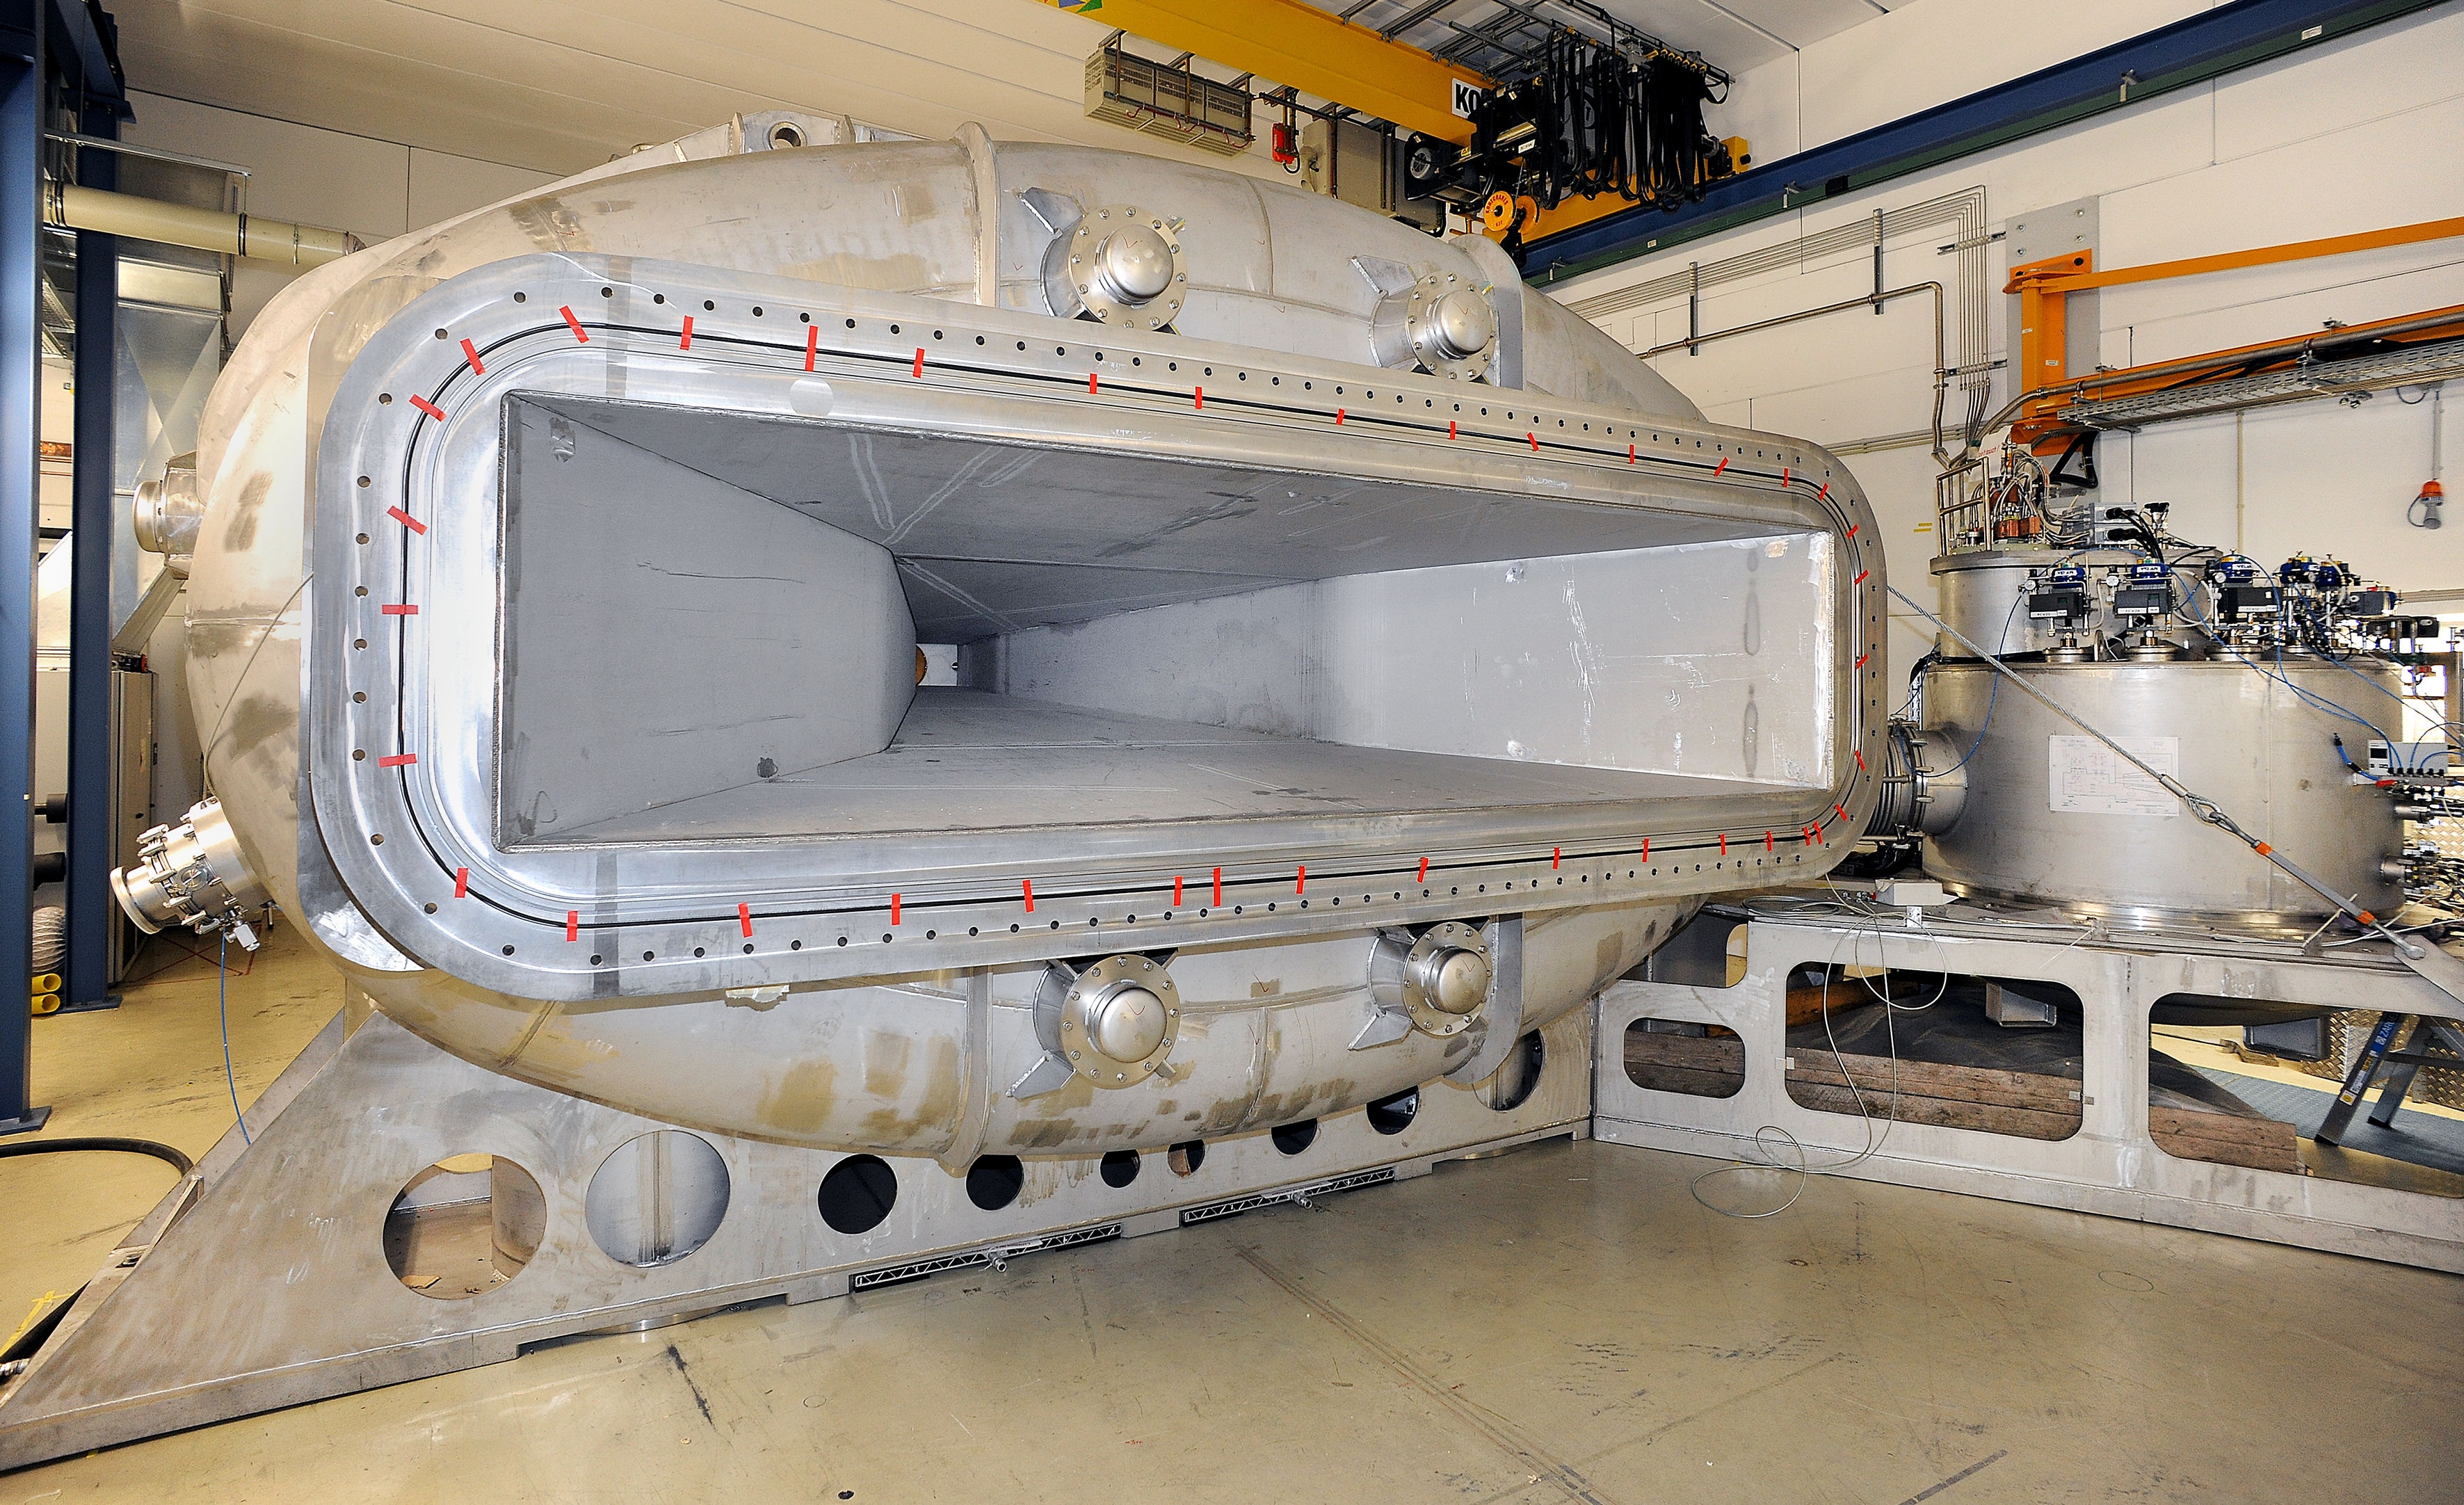
\includegraphics[width=\textwidth,height=6cm,keepaspectratio=true]{Figures/glad_magnet.jpg}
    \caption{
    Upstream view of GLAD magnet in the center of Cave C after installation in February 2016. Picture from \cite{wiki:GLAD} 
    }
    \label{fig:GLAD}
\end{figure}
\subsubsection{CALIFA Calorimeter}\label{sec:califa}
The \textbf{CAL}orimeter for \textbf{I}n \textbf{F}light detection of $\gamma$-rays and high energy charged p\textbf{A}rticles, CALIFA, is one of the main detector components of the R$^3$B setup. It surrounds the target area and covers the full azimuthal range and a polar angular acceptance from 7$^{\circ}$ up to 140$^{\circ}$ in the target region in its final configuration. The calorimeter serves for the detection of gamma rays in the energy region 100 keV $\lesssim$ E$_{\gamma}$ $\lesssim$ 30 MeV and light charged particles, mostly protons, up to E$_p \lesssim$ 700 MeV. To fulfill the demands requested by the different experimental campaigns an energy resolution of $\frac{\Delta E}{E}$ $\sim$ 6\%/$\sqrt(E[\text(MeV)])$ (FWHM) in the gamma-ray energy regime is achieved. For proton energies in the range 100 $\leq \text{E}_p \leq$ 300 AMeV, the corresponding energy resolution is approximately $\frac{\Delta E}{E}$ $\sim$ 1\%/$\sqrt(E[\text(MeV)])$.\newline

\textbf{Geometry}\newline

The CALIFA detector is a highly segmented detector with 2544 CsI(Tl) crystals installed in the final design. Since experiments in the R$^3$B setup operate in relativistic kinematics both the incoming ions as well as the the measured particles originating from reactions experience relativistic effects, more precisely the relativistic Doppler effect. The emitted gamma rays and protons are not isotropically distributed around the source region but are instead boosted in the forward direction. Furthermore, the energy measured in the laboratory frame differs from the kinetic energy in the rest frame of the incoming ion due to relativistic effects.\newline
The relativistic Doppler effect has a huge impact on the geometric design and requirements of CALIFA. Herefore the detector was subdivided into two polar angle ranges~\ref{fig:califa_sec}:
\begin{figure}[htpb]
    \centering
    \includegraphics[width=\textwidth,height=10cm,keepaspectratio=true]{Figures/califa_section_overview.png}
    \caption{
    Schematic view of the Barrel and Endcap(iPhos and CEPA) segments of CALIFA and the according angular and energy distribution of emitted $\gamma$ rays (isotropic and monoenergetic in the projectile frame at beam energy of 700 AMeV). From \cite{tdr:barrel}
    }
    \label{fig:califa_sec}
\end{figure}
\begin{enumerate}
\item BARREL
\begin{itemize}
\item[\ding{108}] $43^{\circ} \leq \theta \leq 140^{\circ}$ - Barrel: This segment covers the region where the lowest rates and energies are expected. The Barrel region contains 1952 CsI(Tl) crystals. The most forward crystals have a length of 22 cm (which allow to stop protons with $E_{kin,p} \leq 315 MeV$). This length is reduced down to 12 cm for the most backward crystals (For more information see Barrel TDR:\cite{tdr:barrel}).   
\end{itemize}
\item ENDCAP
\begin{itemize}
\item[\ding{108}] $19^{\circ} \leq \theta \leq 43^{\circ}$ - Intristic Phoswich (iPhos): In conjunction with the CEPA, the iPhos region forms the CALIFA Endcap. The iPhos region is, same as for the CEPA, affected by high rates. Protons reaching this region have high kinetic energies and therefore a significant fraction of "punch-throughs" is expected. In the iPhos region 480 CsI(Tl) crystals with a length of 22 cm\footnote{To fully stop protons with $E_{kin,p} \approx 600 AMeV$ crystals with a lenght of 60 cm would be needed. Such long crystals would have multiple drawbacks: reduced energy resolution due to worse scintillator light transport, enhanced nuclear reactions inside the crystals and challenging demands on stability of the detector holding structure} are installed and cover each an average polar angle of $\theta \approx$ 3$^{\circ}$.(For more information see Endcap TDR:\cite{tdr:endcap}).
\item[\ding{108}] $7^{\circ} \leq \theta \leq 19^{\circ}$ - CEPA (CALIFA Endcap Phoswich Array): The most forward segment consists of 112 CsI(Tl) crystals. Due to the aforementioned relativistic Doppler effect this area will have the highest intensities and energies. For high beam energies most of the particles will not be stopped inside the crystal and will escape as "punch-throughs". Despite the "punch-through" where ions deposit only a fraction of their kinetic energy ($\Delta E$) in CALIFA, it is possible to reconstruct the initial energy of the particle \footnote{This is done by exploiting the distinct scintillation components of CsI, see more in chapter 5 of \cite{Bendel:98055}}. In CEPA crystals with a length of 22 cm are used, each covering specific polar angle ranges to ensure optimal geometrical coverage. The finer segmentation in the polar angular range provides the advantage of compensating for high event rates while enabling high-resolution Doppler correction.      
\end{itemize}

%\begin{enumerate}
%\item[\ding{108}] $7^{\circ} \leq \theta \leq 19^{\circ}$ - CEPA (CALIFA Endcap Phoswich Array): The most forward segment consists of 112 CsI(Tl) crystals. Due to the aforementioned relativistic Doppler effect this area will have the highest intensities and energies. For high beam energies most of the particles will not be stopped inside the crystal and will escape as "punch-throughs". Despite the "punch-through" ions deposit only a fraction of their kinetic energy ($\Delta E$) in CALIFA it is possible to reconstruct the initial energy of the particle \footnote{This is done by exploiting the distinct scintillation components of CsI, see more in chapter 5 of \cite{Bendel:98055}}. In CEPA crystals with a length of 15 cm are used and cover each a polar angle of $\approx$ 2$^{\circ}$. The finer segmentation in the polar angular range provides the advantage of compensating for high event rates while enabling high-resolution Doppler correction.      
%\item[\ding{108}] $19^{\circ} \leq \theta \leq 43^{\circ}$ - Intristic Phoswich (iPhos): In conjunction with the CEPA, the iPhos region forms the hindmost part of the CALIFA Endcap. The iPhos region is, same as for the CEPA, affected by hight rates. Protons reaching this region have high kinetic energies ($E_{kin,p} \leq 600 MeV$) and herefore a large fraction of "punch-throughs" are expected. In the iPhos region 480 CsI(Tl) crystals with a length of 22 cm\footnote{To fully stop protons with $E_{kin,p} \approx 600 AMeV$ crystals with a lenght of 60 cm would be needed. Such long crystals would have multiple drawbacks: reduced energy resolution due to worse scintillator light transport, enhanced nuclear reactions inside the crystals and challenging demands on stability of the detector holding structure} are installed and cover each a polar angle of $\approx$ 3$^{\circ}$.(For more information see Endcap TDR:\cite{tdr:endcap}).
%\item[\ding{108}] $43^{\circ} \leq \theta \leq 140^{\circ}$ - Barrel: This segment covers the region where the lowest rates and energies are expected. The Barrel region contains 1952 CsI(Tl) crystals. The most forward crystals have a length of 22 cm (which allow to stop protons with $E_{kin,p} \leq 315 MeV$). This length is reduced down to 12 cm for the most backward crystals (For more information see Barrel TDR:\cite{tdr:barrel}).   
%\end{enumerate}
\end{enumerate}
The crystals are arranged in groups of four in one carbon fibre alveolus with a nominal wall thickness of 230 $\mu m$\cite{tdr:barrel} that provide a support structure for the crystals and keep the material budged as low as possible. The alveoli in turn are hold and covered by individual aluminium tiles. From the backside the volume enclosed by the alveoli and the aluminium tiles is flooded with nitrogen to keep humidity low on the surface of the crystals. For a sufficient suspension of the aluminium cover a robust external holding structure was designed, see figure \ref{fig:califa_holding_structure}.\newline
\begin{figure}
    \centering
    \includegraphics[width=\textwidth,height=10cm,keepaspectratio=true]{Figures/hec_zeitrausch.jpeg}
    \caption{ 
	Simulated view of the R\textsuperscript{3}B setup installed in the High-Energy Cave (HEC) at FAIR. The support structures for the CALIFA detector are shown in yellow and green in the lower left part of the image. \textcopyright{} GSI/FAIR, Zeitrausch.
    }
    \label{fig:califa_holding_structure}

\end{figure}
In 2019 CALIFA was for the first time integrated into the R$^3$B setup in form of the CALIFA demonstrator, a prototype consisting of seven mechanically separate petals, each of it containing a set of 64 crystals.\newline
At the end of 2019 the CALIFA frame in its final design was installed and the forward barrel part ($43^{\circ} \leq \theta \leq 90^{\circ}$ and full azimuthal coverage) was equipped with 1024 crystals.\newline
For the S444 and the S467 experiment in 2020 CALIFA was equipped with 180 more crystals in the iPhos region ($19^{\circ} \leq \theta \leq 43^{\circ}$) which corresponds to a coverage of 37.5 \% in azimuthal angle for that region. Right before the S455 fission experiment \cite{grana2023fission} the full installation of the iPhos region was completed.\newline
In February 2024 the full CEPA region ($7^{\circ} \leq \theta \leq 19^{\circ}$) with 112 crystals was commissioned for the first time together with a new equipped part of the backward barrel ($90^{\circ} \leq \theta \leq 102.5^{\circ}$, 128 crystals).\newline   
\textbf{Energy and particle reconstruction with CsI(Tl) scintillator crystals}\newline
Scintillator material, as caesium iodide doped with thallium CsI(Tl), is widely used in experimental physics to detect ioinizing radiation from $\gamma$- rays or charged particles. A comprehensive overview of scintillation mechanisms and the corresponding models can be found in Ref.~\cite{bendel2014entwicklung} and more detailled literature in Refs.~\cite{murray1961scintillation,zazubovich2001physics}.\newline
Thallium-doped Cesium Iodide produces light with a peak emission around 550 nm (green light) and has a high light output\footnote{The light output per MeV deposited energy in CsI(Tl), measured in \cite{holl1988measurement}, resulted in  $5.2\cdot10^{4}$ (scintillation) photons/MeV.}. The high density of CsI with 4.51 g/cm$^3$ makes it to an optimal scintillator material to efficiently absorb $\gamma$- rays and high-energy particles. Moreover the CsI(Tl) crystal is well transparent to its own scintillation light, which is essential for the transport and consequent  detection of the scintillator light. CsI(Tl) crystals are in addition relatively robust compared to other crystals and only slightly hygroscopic making them suitable for long-term use in experimental setups.\newline
In a first approximation, the total amount of emitted light is proportional to the energy deposited in the scintillator. For $\gamma$ -rays this is valid for E$_{\gamma} \gtrsim 400 keV$\cite{syntfeld2007non}. However, for charged particles significant deviations from linearity are observed, a so-called \textit{quenching}\cite{murray1961scintillation}.\newline
Although the the energy calibration of CsI(Tl) crystals for charged particles is challenging, CsI(Tl) as such  has the benefical property of having a complex time dependend light emission consisting of multiple distinct exponential components. The dominant time dependend light emission response of CsI(Tl) $L(t)$ can be approximated as:
\begin{equation}
L(t) = \frac{N_f}{\tau_s} exp(-\frac{t}{\tau_f}) + \frac{N_s}{\tau_s} exp(-\frac{t}{\tau_s})
\end{equation}
Where $N_{f}$ is the amplitude of the fast component and $N_{s}$ the amplitude of the slow component. Accordingly $\tau_{f}$ the life time of the fast component ($\tau_{f} \approx 650-770 ns$ ) and $\tau_{s}$ the lifetime of the slow component ($\tau_{s} \approx 3.2 - 3.5\mu s$). It has been found that the proportion between the two components is energy and particle dependend. This property can be used to identify isotopes by extracting the $N_{f}$ and $N_{s}$ values from pulse shape anaylsis (PSA) on the according light emission response\footnote{The method has been implemented in the CALIFA Firmware as $Quick Particle Identification -QPID$. For more information see \cite{winkel2011implementierung} and \cite{winkel2016komplexe}}, as shown in figure \ref{fig:qpid_califa}.\newline  
\begin{figure}[htpb]
    \centering
    \includegraphics[width=\textwidth,height=10cm,keepaspectratio=true]{Figures/qpid_plot.png}
    \caption{
    Quick Particle Identification(QPID) via fast and slow component $N_{f} / N_{f}$. Each correlation band corresponds to a nuclide, from Ref.\cite{winkel2016komplexe}.
    }
    \label{fig:qpid_califa}
\end{figure}

\textbf{From scintillator light to electrical signal}\newline
The scintillator light produced at different points inside the crystal has first to be transported to the back-end of the crystal. The optimum design has been determined to be frustrum-shaped crystals, wrapped into enhanced specular reflector (ESR) foil which provides excellent reflectivity.\footnote{Detailed information about the crystal wrapping and LAAPD gluing can be found in this work:\cite{hartigevolution}}. Finally, a large-area avalanche photodiode (LAAPD), specifically the Hamamatsu S12102 model~\cite{hamamatsuS8664}, is attached at the rear end of each crystal to enable the detection of scintillation light. Avalanche photodiodes (APDs) operate on the same fundamental principle as conventional photodiodes, converting scintillation light into electrical signals. Both offer the advantage of being insensitive to magnetic fields, making them particularly suitable for applications in environments with strong magnetic interference. As a result of an additional highly doted p-layer a region with very high field is formed which accounts for amplification factors up to $\approx$ 100.\newline
For the next amplification step the  electric signal is forwarded via thin coaxial cables to the front-end of the preamplifiers from Mesytec\cite{mesytec-home} which can serve up to 32 input channels. For CALIFA two general types of peramplifiers are in use:
\begin{enumerate}
\item Dual Range (DR) Preamplifiers: They are used in the iPhos and CEPA region where both high energetic protons as well as gammas are expected. They cover two output signals in parallel: a $gamma$ signal high amplification and a $proton$ signal with  11x lower amplification. Following from this they have 64 channel differential signal output.
\item Single Range (SR) Preamplifiers: In the Barrel region, where only one amplification range is implemented. Depending on the experimental demands these preamplifiers can be switched to $gamma$ or $proton \enspace range$. These peamplifiers have a 32 channel differential signal output.
\end{enumerate}
The fall time for the preamplifiers has been chosen to $\tau_{RC} \approx$ 35 $\mu$s. This is a trade-off between the ballistic deficit on one side (reduction of the signal amplitude due to low $\tau_{RC}$, see also \cite{winkel2011implementierung}, chapter 3.4.5) and rate capability (restricted by large $\tau_{RC}$ value) on the other side.\newline
The differential signal output of the preamplifiers is then transmitted over shielded and twisted line pairs to the input of the FEBEX Addon Boards (FAB) for further processing.\newline
\textbf{Signal Processing and readout system}\newline
The central hardware module for the signal processing in CALIFA is the FEBEX 3B Module (Front End Board with optical link EXtension\footnote{See the FEBEX3b datasheet provided by GSI: \url{https://www.gsi.de/fileadmin/EE/Module/FEBEX/febex3b.pdf} (accessed April 30, 2025).}). Attached on it is a so-called AddOn board developed by TUM. The signal from the preamplifier gets here first filtered by a low pass two pole bessel filter (with cutoff frequency $f_{3dB} = 16 MHz$). Furthermore, since the input of the FEBEX ADCs cover a range of $\pm$ 0.9 V while the signal output from the preamplifier only has one polarity, an offset to the signal is applied to use the full range of the 14 bit flash ADCs. The signal from the ADCs is read out continuously to ring buffers implemented in a FPGA TODO"dip" on the FEBEX card and split up into two branches:\newline
\begin{enumerate}
\item Fast/trigger branch: After being fed to a digital trapezoidal filter the signal is examined by three leading edge discriminators with configurable thresholds. Depending on the experimental requirements a coincident matrix between one or more discriminators and optionally external triggers validates the signal as event ready for data recording.
\item Slow branch: Validated signals then undergo a digital analysis. A pulse shape analysis is performed via various steps - signal decimation, moving average unit -technique, baseline substraction and moving window deconvolution (MWD) - to recall the major steps\footnote{A really detailled description of the pulse shape analysis in CALIFA can be found in Philipp Klenze's\cite{pklenze} and Max Winkel's thesis\cite{winkel2016komplexe}.}. From the resulting pulse shape pulse height measurement the energy deposited in the scintillator is determined. In addition the algorithm for the quick particle identification (QPID) is applied on the incoming signal which provides the fast($N_{f}$) and slow($N_{s}$) component of the signal for isotope identification and differentiation of stopped and punch-through patricles. The CALIFA Firmware also allows to make time over threshold (TOT) measurements which is convenient for energy reconstruction when the incoming signals exceed the ADC range (which might happen when the preamplifier is set to $gamma \enspace range$)\footnote{The TOT energy-reconstruction method has the drawback of being really sensitive to pile-up events overestimating the energy deposition. Hence more suitable for regions with low event rates, such as Barrel region.}.
\end{enumerate}

\textbf{Trigger Distribution and Validation}\newline
The central hub for internal and external trigger forwarding is formed by the Exploder modules\footnote{See the EXPLODER2a datasheet provided by GSI: \url{https://www.gsi.de/fileadmin/EE/Module/EXPLODER/exploder2a\_v5.pdf}(accessed April 30, 2025).}. The FEBEX crates are connected to the Exploder via an eight-fold flat cable known as the trigger bus. This setup allows efficient distribution and handling of trigger signals within the system.\newline
The Exploder module provides multiple input and output lines and includes an internal, switchable bypass matrix. This enables to operate the CALIFA calorimeter in different modes:
\begin{itemize}
\item \textbf{Free-running mode:}internal validation based solely on signal thresholds from the preamplifiers. This configuration is suitable for calibration tasks (e.g., with $\gamma$-ray sources like $^{22}$Na or $^{60}$Co) or low event-rate experiments.
\item \textbf{Externally validated mode:}additional validation signals, such as clean CFD outputs from subdetectors (e.g., START), are used for triggering/event selection. This configuration is preferred for high-rate or coincidence experiments involving multiple detector subsystems.
\end{itemize}
\textbf{Readout Electronics and Data Transfer\footnote{A more detailed explanation about the readout system and the critical FEBEX timing topic can be found in Philipp Klenze's thesis \cite{pklenze}.}}\newline
Trigger bus control between the data acquisition PCs and the FEBEX cards is managed by the TRIXOR card \footnote{See the TRIXOR datasheet provided by GSI: \url{https://www.gsi.de/fileadmin/EE/Module/TRIXOR/trixor.pdf}(accessed April 30, 2025).}, which is directly connected to the the DAQ PCs. It interfaces with both the Exploder modules and the KNIPEX (PCIe Optical Link Interface \footnote{See the KNIPEX datasheet provided by GSI: \url{https://www.gsi.de/fileadmin/EE/Module/Dokumente/kinpex1\_pcb15.pdf} (accessed April 30, 2025).}) card. Connections are established via:
\begin{itemize}
\item ECL lines (TRIXOR $\leftrightarrow$ Exploders)
\item 26-fold flat cable (TRIXOR $\leftrightarrow$ KNIPEX)
\end{itemize}
The KNIPEX card handles high-speed data transfer between the FEBEX electronics and the acquisition computers. It connects to the FEBEX crates via optical fiber and buffers data locally in a 576 MB Reduced Latency Dynamic Random Access Memory (RLDRAM, see Ref.~\cite{jacob2008memory}). The buffered data is then transferred to the PC’s RAM via Direct Memory Access (DMA) with speeds up to 560 MB/s.\newline
Each FEBEX channel is equipped with two memory banks and can store up to 254 events locally. To prevent dead time during readout, a memory bank switch is triggered automatically when one bank reaches its configured event limit. This design ensures continuous, dead-time-free event recording at the channel level. Once a FEBEX channel reaches its threshold, the entire crate is read out synchronously.\newline
\textbf{Data Acquisition System: MBS}\newline
The Multi Branch System (MBS)~\cite{mbsweb}, developed at GSI Helmholtz Center for Heavy Ion Research, is employed on the data acquisition PCs. MBS is a modular software framework that controls detector readout, manages data storage, and provides networking capabilities for distributed acquisition systems.\newline
Key features of MBS include:
\begin{itemize}
\item Integration of multiple detectors into a single, synchronized data stream
\item Trigger signal and dead time exchange via a dedicated trigger bus
\item Time-sorted event building through the \textit{MBS event builder}, which brings together data across detector subsystems into coherent events
\end{itemize}
This system ensures robust, synchronized acquisition for complex multi-detector experiments.


%Central hub for internal and external trigger forwarding are the Exploder modules\footnote{See the EXPLODER2a datasheet provided by GSI: \url{https://www.gsi.de/fileadmin/EE/Module/EXPLODER/exploder2a\_v5.pdf}(accessed April 30, 2025).}. The FEBEX crates are connected over an eight fold flat cable to the Exploder to the triggerbus. The trigger bus between the data acquisition PCs and the FEBEX cards is controlled by the TRIXOR card\footnote{See the TRIXOR datasheet provided by GSI: \url{https://www.gsi.de/fileadmin/EE/Module/TRIXOR/trixor.pdf}(accessed April 30, 2025).}. This card sits inside the data acquisition PCs and is connected via ECL-lines to the Exploders and the KNIPEX (PCIe Optical Link Interface \footnote{See the KNIPEX datasheet provided by GSI: \url{https://www.gsi.de/fileadmin/EE/Module/Dokumente/kinpex1\_pcb15.pdf} (accessed April 30, 2025).}) card via 26 fold flat cable. The KNIPEX card is responsible for the data transfer between FEBEX cards and the data aquisition PCs. It is connected via glas fibre cables to the FEBEX crates and stores locally in a 576 MB large RLDRAM (Reduced Latency Dynamic Random Access Memory, see Ref.~\cite{jacob2008memory}) the data which conecutively gets transmitted  via DMA (Direct Memory Access - data transmission speed up to 560 MB/s) to the RAM of the data acquisition Pcs.\newline
%Since the Exploder provides various input and output lines and an internal switchable bypass matrix the CALIFA calorimeter can be operated as free running system with internal event validation only or by (additional) external validation. In case of internal validation only the signal from the preamplifiers has to exceed predefined threshold(s) to be accepted. This kind of configuration can be used for  the purpose of calibration (with $\gamma$-ray sources like $^{22}$Na or $^{60}$Co) and expected low event rate experiments. For high event rates and event coincidence with other subdetectors additional external validation (e.g. clean CFD signal from START detector) is implemented.\newline
%To overcome dead time initiated by the readout/data transmission procedure each FEBEX channel allows to store up to 254 recoded events on the local memory. Each FEBEX channel has two available memory banks. Whenever one FEBEX channel reaches its preconfigured maximum number of events the full FEBEX crate is read out. To avoid dead time all channels force a  memory bank switch thus allowing  continuous  dead time free event recording.\newline
%The Multi Branch System (MBS), developed at the GSI Helmholtz Center for Heavy Ion Research, is used on the data acquisition PCs. This software consists of several components that control and read out detectors, store the data, or forward it via various network protocols. The system also allows for the joint readout of multiple systems. For this, the trigger modules (TRIXOR) are connected via a special trigger bus to exchange trigger signals and dead time information. The triggered data is then collected, time sorted and cross-detector events are build by the dedicated MBS event builder\footnote{A more detailed explanation about the readout system and the critical FEBEX timing topic can be found in Philipp Klenze's thesis \cite{pklenze}.}. 

\subsubsection{Sofia Time of Flight Wall}
The Sofia Time of Flight Wall (or "Stop detector") is positioned at the very end of the heavy-ion flight-path downstream of the GLAD magnet, behind the MWPC 3 (see subsection~\ref{sec_mwpcs}), at approximately 6.6 m distance from the target position. It consists of a plane of 28 vertically aligned scintillator bars, each of dimension 32x600x5 mm. The scintillator plastics are numbered from 0 to 27 from left to right (when looking in beam direction). The time of flight of the ions between Start and ToFW can be measured by substracting the time measurement of  the Start detector from the ToFW. In optimal operating conditions, the combined time resolution of the Start and ToFW detectors can reach $\sigma_{tot} < 40$ps, enabling precise time-of-flight measurements, for an average time of flight of 30 ns\cite{martin2021fission}. For the technical specifications of the Sofia ToFW, see figure~\ref{fig:sof_tofw_pic} and reference \cite{bail2011time}.

\begin{figure}[htbp]
    \centering
    % The figure (image)
    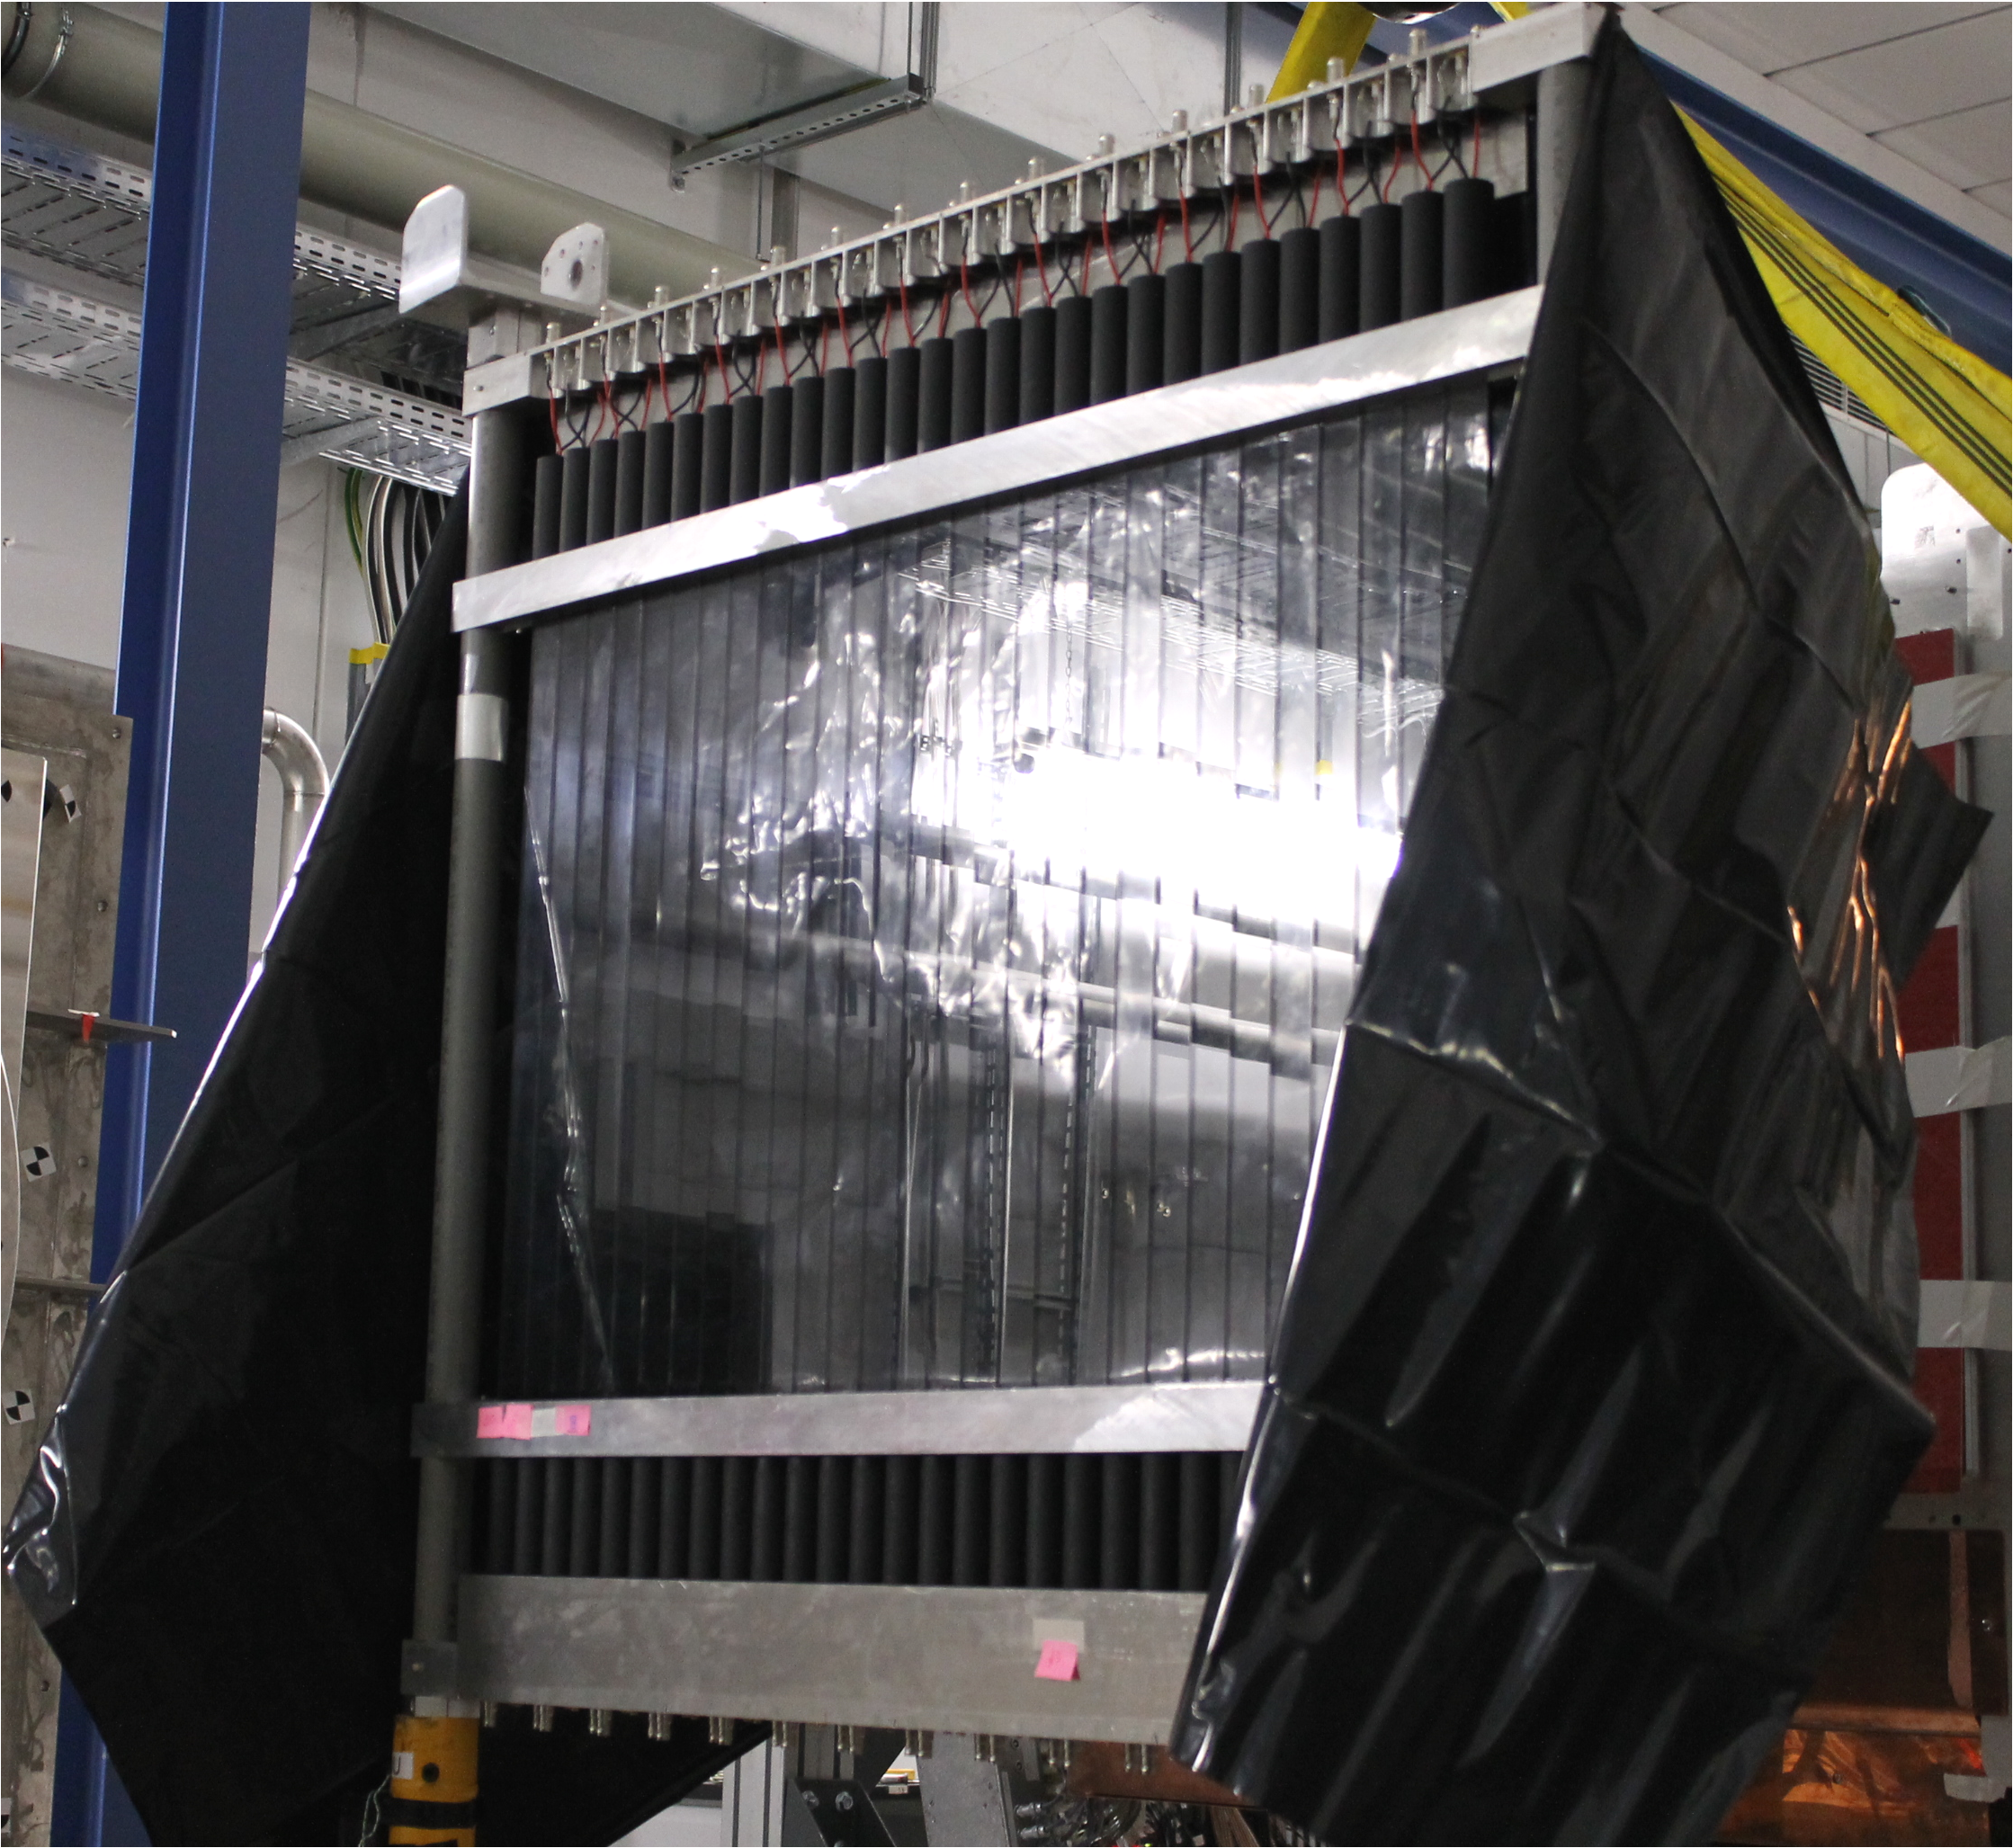
\includegraphics[width=0.7\textwidth]{Figures/sof_tofw.png}

    \vspace{1em} % optional space between image and table

    % The table
	\begin{tabular}{cc}\hline 
  	Plastic & EJ-232, no quencher \\ 
  	Plastic dimensions & 5x32x600 mm$^3$ \\
  	Detector dimension & 5x900x600 mm$^3$ (28 plastics) \\ 
  	Photo-multiplier tubes &  Hamamatsu 6533 and 10580 \\
  	Total number of PMTs & 56 (two per plastic - top and bottom) \\ \hline 
  	\end{tabular}

    % Unified caption for both
    \caption{Sofia ToFW in Cave C, from \cite{martin2021fission}, and technical specifications.}
    \label{fig:sof_tofw_pic}
\end{figure}


\subsubsection{NeuLAND Detector}
For the detection of neutrons emitted from the forward going fragments  the \textbf{N}ew \textbf{L}arge-\textbf{A}rea \textbf{N}eutron \textbf{D}etector (\textbf{NeuLAND}) is installed at zero degrees after GLAD. In its final design it will consist of 30 double planes with each 100 plastic scintillators of size 5x5x250 cm$^3$ providing an active detector surface of 2.5x2.5 m$^2$ and thickness of 3m. Its high detection efficiency, a time resolution of $\sigma_t \le 150 ps$ and high multi-neutron efficiency are crucial detector features for complete kinematics experiments at R$^3$B. A comprehensive analysis of the detector's resolution and efficiency is provided in Refs.~\cite{boretzky2021neuland, boretzky2014neuland}.\newline
For the S444 commissioning experiment in 2020 13 double-planes of the NeuLAND detector have been used. 
\newpage


